\documentclass[oneside,12pt,a4paper]{report}

\usepackage{template}

%chktex-file 8

\begin{document}

    \begin{center}
        \fontsize{17.28}{17.28}
            \textbf{SME0340 - Equações Diferenciais Ordinárias}

            \textbf{Primeira Lista de Exercícios}
    \end{center}

    \vspace{1.5cm}

    \noindent\textbf{\hyperlink{resp:ex1}{\hypertarget{quest:ex1}{Exercício 1}}} (Zill - Seção 1.1, Exercícios 1-8): Classifique as equações diferenciais quanto à sua ordem e linearidade.
    \begin{multicols}{2}
        \begin{enumerate}[label=\alph*)]
            \item $(1-x)y''-4xy'+5y=\cos(x)$
            \item $\dfrac{d^2u}{dr^2}+\dfrac{du}{dr}+u=\cos(r+u)$
            \item $t^5y^{(4)} - t^3y'' + 6y = 0$
            \item $x\dfrac{d^3y}{dx^3} - \left(\dfrac{dy}{dx}\right)^4 + y = 0$
            \item $\dfrac{d^2y}{dx^2} = \sqrt{1 + \left(\dfrac{dy}{dx}\right)^2}$
            \item $\ddot{x} - \left(1 - \dfrac{\dot{x}^2}{3}\right)\dot{x} + x = 0$
            \item $(\sin(\theta))y''' - (\cos(\theta))y' = 2$
            \item $\dfrac{d^2R}{dt^2} = -\dfrac{k}{R^2}$
        \end{enumerate}
    \end{multicols}
    \vspace{0.5cm}

    \noindent\textbf{\hyperlink{resp:ex2}{\hypertarget{quest:ex2}{Exercício 2}}} (Zill - Seção 1.1, Exercícios 11-13): Verifique que a função indicada é solução da equação diferencial dada. Admita um intervalo de definição apropriado $I$.
    \begin{enumerate}[label=\alph*)]
        \item $2y' + y = 0; \quad y = e^{-x/2}$
        \item $y'' + y = \tan(x); \quad y = -(\cos(x)) \ln(\sec(x) + \tan(x))$
        \item $y'' - 6y' + 13y = 0; \quad y = e^{3x} \cos(2x)$
        %\item $\dfrac{dy}{dx} + 20y = 24; \quad y = \dfrac{6}{5} - \dfrac{6}{5}e^{-20t}$
    \end{enumerate}
    \vspace{0.5cm}

    \noindent\textbf{\hyperlink{resp:ex3}{\hypertarget{quest:ex3}{Exercício 3}}} (Zill - Seção 1.1, Exercício 19): Verifique que a expressão indicada é uma solução implícita da equação diferencial dada. Encontre pelo menos uma solução explícita $y=\phi(x)$. Encontre o intervalo de definição $I$ da solução $\phi$. 
    \begin{equation*}
        \frac{dX}{dt}=(X-1)(1-2X); \quad \ln\left(\frac{2X-1}{X-1}\right)=t
    \end{equation*}
    \vspace{0.5cm}

    \noindent\textbf{\hyperlink{resp:ex4}{\hypertarget{quest:ex4}{Exercício 4}}} (Zill - Seção 1.1, Exercícios 21 e 24): Verifique que a família de funções indicada é uma solução da equação diferencial dada. Admita um intervalo de definição $I$ apropriado para cada solução.
    \begin{enumerate}[label=\alph*)]
        \item $\dfrac{dP}{dt} = P(1 - P); \quad P = \dfrac{c_1e^t}{1 + c_1e^t}$
        \item $\dfrac{dy}{dx} + 2xy = 1; \quad y = e^{-x^2} \displaystyle\int_0^x e^{t^2} dt + c_1e^{-x^2}$
    \end{enumerate}
    \vspace{0.5cm}

    \noindent\textbf{\hyperlink{resp:ex5}{\hypertarget{quest:ex5}{Exercício 5}}} (Zill - Seção 1.1, Exercício 26): Sabe-se que $y=\phi_1(x)=\sqrt{25-x^2}$ e $y=\phi_2(x)=-\sqrt{25-x^2}$ são soluções da equação diferencial $\dfrac{dy}{dx}=-\dfrac{x}{y}$ no intervalo $(-5, 5)$. Explique por que a função definida por partes
    \begin{equation*}
        y = \begin{cases}
            \sqrt{25-x^2}, & -5 < x < 0 \\
            -\sqrt{25-x^2}, & 0 \leq x < 5
            
        \end{cases}
    \end{equation*}
    não é uma solução da equação diferencial no intervalo $(-5, 5)$.
    \vspace{0.5cm}

    \noindent\textbf{\hyperlink{resp:ex6}{\hypertarget{quest:ex6}{Exercício 6}}} (Zill - Seção 1.2, Exercícios 3 e 6):
    Sabemos que $y=1/(x^2+c)$ é uma família a um parâmetro de soluções da ED de primeira ordem $y'+2xy^2=0$. Encontre a solução de primeira ordem do PVI formado por esta equação diferencial e pela condição inicial fornecida nos itens. Indique o maior intervalo $I$ para o qual a solução é definida.
    \begin{multicols}{2}
        \begin{enumerate}[label=\alph*)]
            \item $y(2)=\dfrac{1}{3}$
            \item $y\left(\dfrac{1}{2}\right)=-4$
        \end{enumerate}
    \end{multicols}
    \vspace{0.5cm}

    \noindent\textbf{\hyperlink{resp:ex7}{\hypertarget{quest:ex7}{Exercício 7}}} (Zill - Seção 1.2, Exercícios 18, 22 e 23): Determine uma região do plano $xy$ na qual a equação diferencial dada tenha uma única solução cujo gráfico passe pelo ponto $(x_0,y_0)$ nessa região.
    \begin{multicols}{3}
        \begin{enumerate}[label=\alph*)]
            \item $\dfrac{dy}{dx}=\sqrt{xy}$
            \item $(1+y^3)y'=x^2$
            \item $(x^2+y^2)y'=y^2$
        \end{enumerate}
    \end{multicols}
    \vspace{0.5cm}

    \noindent\textbf{\hyperlink{resp:ex8}{\hypertarget{quest:ex8}{Exercício 8}}} (Zill - Seção 1.2, Exercício 30): 
    \begin{enumerate}[label=\alph*)]
        \item Verifique que $y=\tan(x+c)$ é uma família a um parâmetro de soluções da equação diferencial $y'=1+y^2$.
        \item Uma vez que $f(x,y)=1+y^2$ e $\dfrac{\partial f}{\partial y}=2y$ são contínuas, a região $R$ do Teorema de Existência e Unicidade pode ser tomada como o plano $xy$. Use a família de soluções do item (a) para encontrar uma solução explícita do problema de valor inicial de primeira ordem $y'=1+y^2$, $y(0)=0$. Mesmo estando $x_0=0$ no intervalo $-2<x<2$, explique por que a solução não está definida nesse intervalo.
        \item Determine o maior intervalo $I$ de definição da solução do priblema de valor inicial do item (b).
    \end{enumerate}
    \vspace{0.5cm}

    \noindent\textbf{\hyperlink{resp:ex9}{\hypertarget{quest:ex9}{Exercício 9}}}: Considere o PVI

    \[
    \begin{cases} 
    \frac{dy}{dt} = f(t,y) + g(t,y) \\ 
    y(2) = \frac{\pi}{2}
    \end{cases}
    \]

    \noindent Determine todas as soluções para o PVI, sabendo que $f^2(t,y) + g^2(t,y) = \cos^2(y)$ para todo $(t,y) \in \mathbb{R}^2$, e que $f, g \in C^1$.
    \vspace{0.5cm}

    \noindent\textbf{\hyperlink{resp:ex10}{\hypertarget{quest:ex10}{Exercício 10}}}: Seja $f:\mathbb{R}^n \to \mathbb{R}^n$ de classe $C^1$ e suponhamos que $\phi(t)$, definida em $\mathbb{R}$, seja solução da EDO

    \[
    \begin{cases} 
    y' = f(y)\\ 
    y(t_0) = y_0
    \end{cases}
    \]

    \noindent É possível que existam $t_1, t_2 \in \mathbb{R}$, $t_1\neq t_2$, tais que $\phi(t_1) = \phi(t_2)$ mas $\phi'(t_1) \neq \phi'(t_2)$?
    \vspace{0.5cm}
    
    \noindent\textbf{\hyperlink{resp:ex11}{\hypertarget{quest:ex11}{Exercício 11}}}: Suponha que uma população humana com quantidade de indivíduos $P(t)$ viva em um ambiente qualquer.
    \begin{enumerate}[label=\alph*)]
        \item Assumindo que a variação da população é diretamente proporcional ao número de indivíduos, determine a equação diferencial que descreve esse modelo de crescimento.
        \item Agora, além de assumir que a variação da população é proporcional a $P(t)$, assuma também que o ambiente é capaz de suportar uma quantidade máxima de indivíduos $K$. Qual é a equação diferencial que descreve esse novo modelo?
        \item (Zill - Seção 1.3, Exercício 2): Em um outro modelo de variação populacional de uma comunidade supõe-se que a taxa segundo a qual a população varia é uma taxa \textit{líquida} - isto é, a diferença entre a taxa de natalidade e a taxa de mortalidade na comunidade. Determine um modelo para uma equação diferencial que governe a evolução da população $P(t)$, se as taxas de natalidade e mortalidade forem proporcionais à população presente no instante $t>0$.
    \end{enumerate}
    \vspace{0.5cm}
    
    \noindent\textbf{\hyperlink{resp:ex12}{\hypertarget{quest:ex12}{Exercício 12}}} (Zill - Seção 1.3, Exercícios 10-12):
    \begin{enumerate}[label=\alph*)]
        \item Suponha que um grande tanque para misturas contenha inicialmente $300$ galões de água, no qual foram dissolvidas $50$ libras de sal. Uma outra solução de sal é bombeada para dentro do tanque a uma taxa de $3~\mathrm{gal/min}$, e então, quando a solução está bem misturada, é bombeada para fora a uma taxa menor de $2~\mathrm{gal/min}$. Se a concentração da solução que entra for de $2~\mathrm{lb/gal}$, determine uma equação diferencial para a quantidade de sal $A(t)$ no tanque, no instante $t > 0$.
        \item Qual é a equação diferencial no item a), se a solução bem misturada é bombeada a uma taxa de $3.5~\mathrm{gal/min}$?
        \item Generalize o modelo utilizado nos itens anteriores supondo que o tanque grande contém inicialmente $N_0$ galões de solução salina, $r_e$ e $r_s$ são as taxas de entrada e saída, respectivamente (medidas em galões por minuto), $c_e$ é a concentração de sal no fluxo de entrada, $c(t)$ é a concentração de sal no tanque assim como no fluxo de saída em um instante $t$ qualquer (medido em libras de sal por galão), e $A(t)$ é a quantidade de sal no tanque em um instante $t > 0$ qualquer.
    \end{enumerate}
    \vspace{0.5cm}

    \noindent\textbf{\hyperlink{resp:ex13}{\hypertarget{quest:ex13}{Exercício 13}}} (Zill - Seção 1.3, Exercícios 15 e 16):
    \begin{enumerate}[label=\alph*)]
        \item Um circuito em série contém um resistor e um indutor conforme a Figura \ref{fig:circuitoRL}. Determine uma equação diferencial para a corrente $i(t)$ se a resistência for $R$, a indutância for $L$ e a voltagem aplicada for $E(t)$.
        \item Um circuito em série contém um resistor e um capacitor conforme a Figura \ref{fig:circuitoRC}. Determine uma equação diferencial para a carga $q(t)$ no capacitor, se a resistência for $R$, a capacitância for $C$ e a voltagem aplicada for $E(t)$.
    \end{enumerate}

    \begin{figure}[H]
    \centering
    \begin{subfigure}{.45\textwidth}
        \centering
        \begin{circuitikz}
        \draw
        % Fonte de tensão com 'E' no centro
        (0,0) to[esource, n=fonte] (0,2.5)
        
        % Resistor R no topo (l_ coloca o rótulo abaixo do componente)
        (0,2.5) to[L, l_=$L$] (4,2.5)
        
        % Fio fechando o circuito à direita
        (4,2.5) -- (4,0)
        
        % Indutor L na base (l_ coloca o rótulo abaixo do componente, 
        % pois estamos desenhando da direita para a esquerda)
        (4,0) to[R, l=$R$] (0,0);

        \node at (fonte.center) {$E$};
        
        \end{circuitikz}
        \caption{}\label{fig:circuitoRL}
    \end{subfigure}
    \begin{subfigure}{.45\textwidth}
        \centering
        \begin{circuitikz}
        \draw
        % Fonte de tensão com 'E' no centro
        (0,0) to[esource, n=fonte] (0,2.5)
        
        % Resistor R no topo (l_ coloca o rótulo abaixo do componente)
        (0,2.5) to[R, l_=$R$] (4,2.5)
        
        % Fio fechando o circuito à direita
        (4,2.5) -- (4,0)
        
        % Capacitor C na base (l coloca o rótulo abaixo do componente, 
        % pois estamos desenhando da direita para a esquerda)
        (4,0) to[C, l=$C$] (0,0);

        \node at (fonte.center) {$E$};
        
        \end{circuitikz}
        \caption{}\label{fig:circuitoRC}
    \end{subfigure}
    \caption{Circuitos do Exercício 13.}
    \end{figure}

    \noindent\textbf{\hyperlink{resp:ex14}{\hypertarget{quest:ex14}{Exercício 14}}} (Zill - Seção 1.3, Exercício 21): Um pequeno foguete de um estágio é lançado verticalmente. Uma vez lançado, o foguete consome seu combustível e assim sua massa total $m(t)$ varia com o tempo $t > 0$. Se assumirmos que a direção positiva é para cima, a resistência do ar é proporcional à velocidade instantânea $v$ do foguete e $R$ é um empurrão para cima ou força gerada pelo sistema de propulsão, construa um modelo matemático para a velocidade $v(t)$ do foguete. Use a formulação da quantidade de movimento linear da Segunda Lei de Newton, isto é, $F = \dfrac{d}{dt}(mv)$, onde $F$ é a força resultante sobre o foguete.
    \vspace{0.5cm}

    \noindent\textbf{\hyperlink{resp:ex15}{\hypertarget{quest:ex15}{Exercício 15}}} (Zill - Seção 1.3, Exercício 22): No \hyperlink{quest:ex14}{Exercício 14}, a massa $m(t)$ é a soma de três diferentes massas: $m(t) = m_p + m_v + m_f(t)$, onde $m_p$ é a massa constante de carga, $m_v$ é a massa constante do veículo e $m_f(t)$ é a quantidade variável de combustível.
    \begin{enumerate}[label=\alph*)]
        \item Mostre que a taxa com que a massa total $m(t)$ do foguete muda é a mesma taxa com que a massa $m_f(t)$ do combustível muda.
        \item Se o foguete consome seu combustível numa taxa constante $\lambda$, ache $m(t)$. Então reescreva a equação diferencial no \hyperlink{quest:ex14}{Exercício 14} em termos de $\lambda$ e da massa inicial total $m(0) = m_0$.
        \item Sob o pressuposto do item (b), mostre que o tempo de queima $t_b > 0$ do foguete, ou o tempo na qual todo o combustível é consumido é $t_b = m_f(0)/\lambda$, onde $m_f(0)$ é a massa inicial de combustível.
    \end{enumerate}

    %==========================================================================

    \chapter*{Resolução dos Exercícios}

        \begin{tcolorbox}[enhanced, breakable, colback=blue!1!white,colframe=blue!75!black,title=\textbf{\hyperlink{quest:ex1}{\hypertarget{resp:ex1}{Exercício 1}}}]

        \noindent Para que seja linear, a equação diferencial deve ser da forma

        \begin{equation}\label{eq:formalinear}
            a_n(x)\frac{d^ny}{dx^n} + a_{n-1}(x)\frac{d^{n-1}y}{dx^{n-1}} + \cdots + a_1(x)\frac{dy}{dx} + a_0(x)y = g(x)
        \end{equation}

        \noindent Nesse sentido, deve-se analisar a forma de cada item, verificando se ela corresponde àquela da Equação \ref{eq:formalinear}. Além disso quanto à ordem, é necessário analisar aquela da maior derivada presente na equação.
        \tcblower

        \noindent \textcolor{blue}{\textbf{Item a)}} Comparando com a Equação \ref{eq:formalinear}, temos $a_0(x)=5$, $a_1(x)=-4x$, $a_2(x)=(1-x)$ e $g(x)=\cos(x)$. Como todos os termos que multiplicam $y$ e suas derivadas são funções apenas de $x$, a equação é \textbf{linear}. A partir da maior derivada, $y''$, pode-se classificar a equação como de \textbf{segunda ordem}.

        \noindent \textcolor{blue}{\textbf{Item b)}} Observa-se que a variável dependente $u$ aparece dentro da função cosseno na equação. Dessa forma, podemos classificá-la como \textbf{não linear}. A partir da maior derivada, $\dfrac{d^2u}{dr^2}$, podemos classificar a equação como de \textbf{segunda ordem}.

        \noindent \textcolor{blue}{\textbf{Item c)}} A partir da comparação com a Equação \ref{eq:formalinear}, temos $a_0(t)=6$, $a_2(t)=-t^3$, $a_4(t)=t^5$ e $g(t)=0$. Como todos os termos são funções apenas de $t$, a equação é \textbf{linear}. A partir da maior derivada, $y^{(4)}$, pode-se classificar a equação como de \textbf{quarta ordem}.

        \noindent \textcolor{blue}{\textbf{Item d)}} Observa-se que a primeira derivada da variável dependente $y$ aparece elevada à quarta potência na equação. Dessa forma, podemos classificá-la como \textbf{não linear}. A partir da maior derivada, $\dfrac{d^3y}{dx^3}$, podemos classificar a equação como de \textbf{terceira ordem}.
        
        \noindent \textcolor{blue}{\textbf{Item e)}} Observa-se que a primeira derivada da variável dependente $y$ aparece dentro de uma raiz quadrada na equação. Dessa forma, podemos classificá-la como \textbf{não linear}. A partir da maior derivada, $\dfrac{d^2y}{dx^2}$, podemos classificar a equação como de \textbf{segunda ordem}.

        \noindent \textcolor{blue}{\textbf{Item f)}} Podemos rearranjar a equação para obter

        $$\ddot{x}-\dot{x}-\frac{\dot{x}^3}{3}+x=0$$

        \noindent Observa-se que primeira derivada da variável dependente $x$ aparece dentro de um termo cúbico na equação. Dessa forma, podemos classificá-la como \textbf{não linear}. A partir da maior derivada, $\ddot{x}$, podemos classificar a equação como de \textbf{segunda ordem}.

        \noindent \textcolor{blue}{\textbf{Item g)}} Ao comparar com a Equação \ref{eq:formalinear}, temos $a_1(\theta)=-\cos(\theta)$, $a_3(\theta)=\sin(\theta)$ e $g(\theta)=2$. Como todos os termos são funções apenas de $\theta$, a equação é \textbf{linear}. A partir da maior derivada, $y'''$, pode-se classificar a equação como de \textbf{terceira ordem}.

        \noindent \textcolor{blue}{\textbf{Item h)}} Rearranjando a equação, temos

        $$R^2\frac{d^2R}{dt^2}=-k$$

        \noindent Como há um termo $R^2$ multiplicando sua segunda derivada, a equação é \textbf{não linear}. A partir da maior derivada, $\dfrac{d^2R}{dt^2}$, podemos classificar a equação como de \textbf{segunda ordem}.

        \end{tcolorbox}
        
        %%

        \begin{tcolorbox}[enhanced, breakable, colback=blue!1!white,colframe=blue!75!black,title=\textbf{\hyperlink{quest:ex1}{\hypertarget{resp:ex2}{Exercício 2}}}]

        \noindent \textcolor{blue}{\textbf{Item a)}} Para verificar que $y=e^{-x/2}$ é solução da equação diferencial $2y' + y = 0$, devemos calcular a derivada da variável dependente $y$ e substituí-la na equação. Calculando-a, temos
        $$\frac{d}{dx}(y)=\frac{d}{dx}\left(e^{-x/2}\right) = e^{-x/2}\frac{d}{dx}\left(-\frac{x}{2}\right)=-\frac{e^{-x/2}}{2}$$

        \noindent Substituindo $y$ e $y'$ na equação, temos
        $$2\left(-\frac{e^{-x/2}}{2}\right) + e^{-x/2} = 0\Rightarrow-e^{-x/2}+e^{-x/2}=0\Rightarrow\boxed{0=0}$$

        \noindent O que confirma que $y=e^{-x/2}$ é solução da equação diferencial dada. Como a função é definida para todo $x\in\mathbb{R}$, o intervalo de definição da solução é $I=(-\infty, \infty)$.
        
        \noindent \textcolor{blue}{\textbf{Item b)}} Derivando a expressão dada de $y$, temos
        \[y'=\sin(x)\ln(\sec(x)+\tan(x))-\cos(x)\left(\frac{1}{\sec(x)+\tan(x)}\right)\cdot(\tan(x)\sec(x)+\sec^2(x))\]
        \[y'=\sin(x)\ln(\sec(x)+\tan(x))-1\]
        \noindent Derivando novamente, temos
        \[y''=\cos(x)\ln(\sec(x)+\tan(x))+\sin(x)\left(\frac{1}{\sec(x)+\tan(x)}\right)\cdot(\tan(x)\sec(x)+\sec^2(x))\]
        \[y''=\cos(x)\ln(\sec(x)+\tan(x))+\tan(x)\]
        \noindent Substituindo $y$, $y'$ e $y''$ na equação, temos
        \[\cos(x)\ln(\sec(x)+\tan(x))+\tan(x)-\cos(x)\ln(\sec(x)+\tan(x))=\tan(x)\Rightarrow\]
        \[\boxed{\tan(x)=\tan(x)}\]
        \noindent O que confirma que $y=-(\cos(x)) \ln(\sec(x) + \tan(x))$ é solução da equação diferencial dada. O intervalo de definição da solução é obtido tomando o argumento do logaritmo como positivo. Dessa forma, temos
        \[\sec(x)+\tan(x) > 0\Rightarrow\frac{1}{\cos(x)}+\frac{\sin(x)}{\cos(x)} > 0\Rightarrow\frac{1+\sin(x)}{\cos(x)} > 0\]
        \noindent O numerador da fração é sempre positivo. Dessa maneira, tomando os intervalos nos quais $\cos(x)$ é positivo, temos que:
        \[x \in \left(\frac{4k\pi-\pi}{2}, \frac{4k\pi+\pi}{2}\right),~k \in\mathbb{Z}\Rightarrow I=\left(\frac{4k\pi-\pi}{2}, \frac{4k\pi+\pi}{2}\right),~k \in\mathbb{Z}\]

         \noindent \textcolor{blue}{\textbf{Item c)}} A primeira derivada de $y$ é
        \[y' = 3e^{3x}\cos(2x) - 2e^{3x}\sin(2x)=e^{3x}(3\cos(2x)-2\sin(2x))\]
        \noindent Além disso, a segunda derivada de $y$ é
        \[y''=3e^{3x}(3\cos(2x)-2\sin(2x))+e^{3x}(-6\sin(2x)-4\cos(2x))\]
        \[y''=e^{3x}(5\cos(2x)-12\sin(2x))\]
        \noindent Substituindo $y$, $y'$ e $y''$ na equação, temos
        \[e^{3x}(5\cos(2x)-12\sin(2x))-6e^{3x}(3\cos(2x)-2\sin(2x))+13e^{3x}\cos(2x)=0\Rightarrow\boxed{0=0}\]
        \noindent O que confirma que $y=e^{3x} \cos(2x)$ é solução da equação diferencial dada. Como a função é definida para todo $x\in\mathbb{R}$, o intervalo de definição da solução é $I=(-\infty, \infty)$.
    
        \end{tcolorbox}

        %%

        \begin{tcolorbox}[enhanced, breakable, colback=blue!1!white,colframe=blue!75!black,title=\textbf{\hyperlink{quest:ex3}{\hypertarget{resp:ex3}{Exercício 3}}}]
        \noindent Para verificar que a expressão é solução implícita da equação diferencial, devemos diferenciá-la implicitamente em relação à variável independente $t$:
        \begin{gather*}
            \frac{d}{dt}\left(\ln(2X-1)-\ln(X-1)\right)=\frac{d}{dt}(t)\Rightarrow
            \frac{1}{2X-1}\cdot 2\frac{dX}{dt} - \frac{1}{X-1}\cdot \frac{dX}{dt} = 1\Rightarrow\\
            \left(\frac{2}{2X-1} - \frac{1}{X-1}\right)\frac{dX}{dt} = 1\Rightarrow
            -\frac{1}{(2X-1)(X-1)}\frac{dX}{dt} = 1\Rightarrow\\
            \frac{dX}{dt} = -(2X-1)(X-1) \Rightarrow \boxed{\frac{dX}{dt} = (X-1)(1-2X)}
        \end{gather*}

        \noindent A expressão obtida é idêntica à equação diferencial dada, o que confirma que a expressão é uma solução implícita da equação diferencial. Para encontrar uma solução explícita, basta isolar a variável dependente $X$ na expressão dada:
        \begin{gather*}
            \ln\left(\frac{2X-1}{X-1}\right)=t\Rightarrow
            \frac{2X-1}{X-1}=e^t\Rightarrow
            2X-1 = e^t(X-1)\Rightarrow\\
            2X-1 = e^tX - e^t\Rightarrow
            2X - e^tX = -e^t + 1\Rightarrow
            X(2 - e^t) = 1 - e^t\Rightarrow\\
            \boxed{X = \frac{1 - e^t}{2 - e^t}}
        \end{gather*}

        \noindent Por fim, para obter o intervalo de definição da solução, devemos analisar o denominador da solução explícita, que deve ser diferente de $0$, e o termo dentro do logaritmo da solução implícita, que deve ser sempre maior que $0$. Dessa forma:

        $$2-e^t \neq 0 \Rightarrow e^t \neq 2 \Rightarrow t \neq \ln(2)$$

        \noindent Substituindo a solução explícita no argumento do logaritmo na solução implícita, temos:

        $$\frac{2\frac{1-e^t}{2-e^t}-1}{\frac{1-e^t}{2-e^t}-1}=\frac{2-2e^t-2+e^t}{1-e^t-2+e^t}=e^t$$

        \noindent Que é positivo para todo $t \in \mathbb{R}$. Dessa forma, podemos definir $I=(-\infty, \ln(2))$ ou $I=(\ln(2), \infty)$.
        
        \end{tcolorbox}

        %%

        \begin{tcolorbox}[enhanced, breakable, colback=blue!1!white,colframe=blue!75!black,title=\textbf{\hyperlink{quest:ex4}{\hypertarget{resp:ex4}{Exercício 4}}}]

            \noindent \textcolor{blue}{\textbf{Item a)}} Tomando a primeira derivada da solução proposta, temos
            \[\frac{dP}{dt} = \frac{c_1e^t(1+c_1e^t)-c_1^2e^{2t}}{(1+c_1e^t)^2} = \frac{c_1e^t}{(1+c_1e^t)^2}\]
            \noindent Substituindo $P$ e $\dfrac{dP}{dt}$ na equação diferencial, temos
            \[\frac{c_1e^t}{(1+c_1e^t)^2} = \frac{c_1e^t}{1+c_1e^t}\left(1-\frac{c_1e^t}{1+c_1e^t}\right)\Rightarrow\boxed{\frac{c_1e^t}{(1+c_1e^t)^2} = \frac{c_1e^t}{(1+c_1e^t)^2}}\]
            \noindent O que confirma que $P = \dfrac{c_1e^t}{1 + c_1e^t}$ é solução da equação diferencial dada. Para encontrar o intervalo de definição da solução, tomamos o denominador da solução como diferente de $0$:
            \[1+c_1e^t \neq 0\Rightarrow e^t \neq -\frac{1}{c_1}\]
            Se $c_1 > 0$, então a condição é satisfeita para todo $t \in \mathbb{R}$. Se $c_1 < 0$, então a condição é satisfeita para todo $t \in \mathbb{R}$, exceto para $t = \ln\left(-\frac{1}{c_1}\right)$. Dessa forma, o intervalo de definição da solução é da forma
            \begin{equation*}
            I=\begin{cases}
                (-\infty, \infty)$ se $c_1 > 0\\
                (-\infty, \ln\left(-\frac{1}{c_1}\right)) \text{ ou } (\ln\left(-\frac{1}{c_1}\right), \infty)$ se $c_1 < 0
            \end{cases}
            \end{equation*}

            \noindent \textcolor{blue}{\textbf{Item b)}} Tomando a primeira derivada da solução fornecida, temos
            \[\frac{dy}{dx} = -2xe^{-x^2}\int_{0}^{x} e^{t^2} dt+e^{-x^2}(e^{x^2}\cdot1-e^0\cdot0)-2xc_1e^{-x^2}\]
            \[\frac{dy}{dx} = -2xe^{-x^2}\int_{0}^{x} e^{t^2} dt+1-2xc_1e^{-x^2}\]
            \noindent Substituindo $y$ e $\dfrac{dy}{dx}$ na equação diferencial, temos
            \[-2xe^{-x^2}\int_{0}^{x} e^{t^2} dt+1-2xc_1e^{-x^2}+2x\left(e^{-x^2}\int_{0}^{x} e^{t^2} dt+c_1e^{-x^2}\right) = 1\Rightarrow\boxed{1=1}\]
            \noindent O que confirma que $y = e^{-x^2} \displaystyle\int_0^x e^{t^2} dt + c_1e^{-x^2}$ é solução da equação diferencial dada. A função encontrada como solução é definida para todo $x \in \mathbb{R}$, o que implica que o intervalo de definição da solução é $I=(-\infty, \infty)$.
        \end{tcolorbox}

        %%

        \begin{tcolorbox}[enhanced, breakable, colback=blue!1!white,colframe=blue!75!black,title=\textbf{\hyperlink{quest:ex5}{\hypertarget{resp:ex5}{Exercício 5}}}]

            \noindent Vamos analisar os limites laterais da função na vizinhança do ponto $0$. Temos que:

            \begin{equation*}
                \begin{cases}
                    \lim_{x\to 0^-} \sqrt{25-x^2} = 5 \\
                    \lim_{x\to 0^+} -\sqrt{25-x^2} = -5
                \end{cases}
            \end{equation*}

            \noindent Como os limites laterais são diferentes, a função não é contínua em $x=0$. Este fato é explicitado na Figura \ref{fig:graficoex5}. Por definição, ela não é diferenciável nesse ponto, o que a invalida como solução da equação diferencial dada no intervalo $I=(-5, 5).$

            \begin{figure}[H]
            \centering
            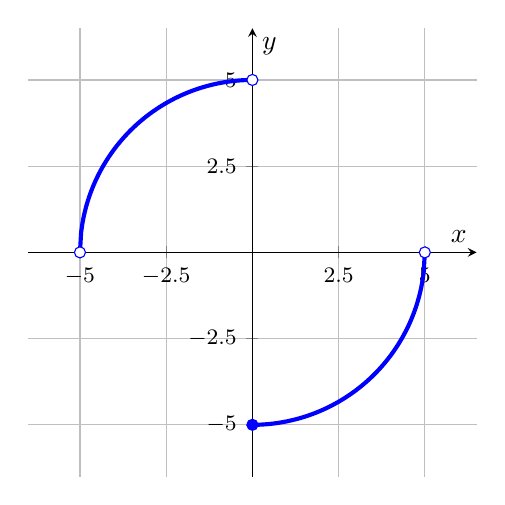
\begin{tikzpicture}
            \begin{axis}[
                axis lines = middle,
                axis equal image, % Mantém a proporção real (círculo não vira elipse)
                xlabel = {$x$},
                ylabel = {$y$},
                xmin = -6.5, xmax = 6.5,
                ymin = -6.5, ymax = 6.5,
                grid = major,
                xtick = {-5,-2.5,0,2.5,5},
                ytick = {-5,-2.5,0,2.5,5},
                tick label style={font=\footnotesize}
            ]

            % --- Primeiro Ramo: raiz(25 - x^2) para -5 < x < 0 ---
            \addplot[domain=-5:0, samples=150, blue, line width=1.5pt] {sqrt(25-x^2)};

            % Bolinhas vazias nos extremos do ramo 1 (x=-5 e x=0)
            \addplot[only marks, mark=*, blue, fill=white] coordinates {(-5,0) (0,5)};


            % --- Segundo Ramo: -raiz(25 - x^2) para 0 <= x < 5 ---
            \addplot[domain=0:5, samples=150, blue, line width=1.5pt] {-sqrt(25-x^2)};

            % Bolinha cheia em x=0 e bolinha vazia em x=5 para o ramo 2
            \addplot[only marks, mark=*, blue] coordinates {(0,-5)};
            \addplot[only marks, mark=*, blue, fill=white] coordinates {(5,0)};
            
            \end{axis}
            \end{tikzpicture}
            \caption{Gráfico de $y$.}\label{fig:graficoex5}
            \end{figure}

        \end{tcolorbox}

        \begin{tcolorbox}[enhanced, breakable, colback=blue!1!white,colframe=blue!75!black,title=\textbf{\hyperlink{quest:ex6}{\hypertarget{resp:ex6}{Exercício 6}}}]

            \noindent\textcolor{blue}{\textbf{Item a)}} Ao utilizar as informações da condição inicial, podemos encontrar o valor de $c$ que soluciona o PVI. Substituindo $x=2$ e $y=\dfrac{1}{3}$ na expressão de $y$, temos
            \[\frac{1}{3} = \frac{1}{2^2+c} \Rightarrow 4+c = 3 \Rightarrow \boxed{c = -1}\]
            \noindent Dessa forma, função que satisfaz o PVI é $y = \dfrac{1}{x^2-1}$. Analisando-a, percebemos que a função não é definida em $x=-1$ e $x=1$. Dessa forma, o maior intervalo de definição da solução que contém a condição inicial especificada é  $I=(1, \infty)$.

            \noindent\textcolor{blue}{\textbf{Item b)}} Substituindo $x=\dfrac{1}{2}$ e $y=-4$ na expressão de $y$, temos
            \[-4 = \frac{1}{\left(\frac{1}{2}\right)^2+c} \Rightarrow \frac{1}{4}+c = -\frac{1}{4} \Rightarrow \boxed{c = -\frac{1}{2}}\]
            \noindent Dessa forma, função que satisfaz o PVI é $y = \dfrac{1}{x^2-\frac{1}{2}}$. Como o denominador deve ser diferente de $0$ para que a função seja definida, encontramos que $x=-\dfrac{1}{\sqrt{2}}$ e $x=\dfrac{1}{\sqrt{2}}$ não fazem parte de seu domínio. Dessa forma, o maior intervalo de definição da solução que contém a condição inicial especificada é  $I=\left(-\dfrac{1}{\sqrt{2}}, \dfrac{1}{\sqrt{2}}\right)$.

        \end{tcolorbox}

        \begin{tcolorbox}[enhanced, breakable, colback=blue!1!white,colframe=blue!75!black,title=\textbf{\hyperlink{quest:ex7}{\hypertarget{resp:ex7}{Exercício 7}}}]

        \noindent\textcolor{blue}{\textbf{Item a)}} Temos uma equação diferencial da forma $y' = f(x,y)$, onde $f(x,y) = \sqrt{xy}$. Para que o T.E.U seja aplicado, é necessário que $f$ e $\dfrac{\partial f}{\partial y}$ sejam contínuas em uma região $R$ do plano $xy$ que contenha o ponto $(x_0, y_0)$.

        \noindent Para que esteja definida em $\mathbb{R}^2$, a condição $xy \geq 0$ deve ser satisfeita. Dessa forma, devemos ter $x \geq 0$ e $y \geq 0$, ou $x \leq 0$ e $y \leq 0$ (ou seja, o primeiro ou terceiro quadrantes). Além disso, a função $\dfrac{\partial f}{\partial y}$ é dada por
        \[\frac{\partial f}{\partial y} = \frac{\partial}{\partial y}(\sqrt{xy}) = \frac{x}{2\sqrt{xy}}\]

        \noindent Analisando o denominador da derivada encontrada, concluimos que $x\neq 0$ e $y\neq0$. Além disso, como o argumento da raiz deve ser positivo, temos que $xy\geq0$. Dessa forma, a maior região $R$ pode ser tomada tal que $R=(0, \infty) \times (0, \infty)$, ou $R=(-\infty, 0) \times (-\infty, 0)$.

        \noindent\textcolor{blue}{\textbf{Item b)}} Tomando $f(x,y) = \dfrac{x^2}{1+y^3}$, temos que a função não é definida em $y=-1$. Além disso, derivando $f$ em relação a $y$, temos
        \[\frac{\partial f}{\partial y} = \frac{\partial}{\partial y}\left(\frac{x^2}{1+y^3}\right) = \frac{-3x^2y^2}{(1+y^3)^2}\]
        \noindent Analisando o domínio de $\dfrac{\partial f}{\partial y}$, temos novamente que a função não é definida em $y=-1$. Dessa forma, a maior região $R$ pode ser tomada como $R=(-\infty, \infty) \times (-1, \infty)$ ou $R=(-\infty, \infty) \times (-\infty, -1)$.

        \noindent\textcolor{blue}{\textbf{Item c)}} Tomando $f(x,y) = \dfrac{y^2}{x^2+y^2}$, temos que a função não é definida no ponto $(x, y)=(0,0)$. Além disso, derivando $f$ em relação a $y$, temos
        \[\frac{\partial f}{\partial y} = \frac{\partial}{\partial y}\left(\frac{y^2}{x^2+y^2}\right) = \frac{2y(x^2+y^2)-y^2(2y)}{(x^2+y^2)^2}=\frac{2x^2y}{(x^2+y^2)^2}\]
        \noindent Analisando o domínio de $\dfrac{\partial f}{\partial y}$, temos novamente que a função não é definida no ponto $(x, y)=(0,0)$. Dessa forma, a região $R$ pode ser tomada como qualquer uma que não contenha a origem.

        \end{tcolorbox}

        \begin{tcolorbox}[enhanced, breakable, colback=blue!1!white,colframe=blue!75!black,title=\textbf{\hyperlink{quest:ex8}{\hypertarget{resp:ex8}{Exercício 8}}}]

        \noindent\textcolor{blue}{\textbf{Item a)}} Derivando a expressão dada de $y$, temos
        \[y' = \left(\frac{\sin(x+c)}{\cos(x+c)}\right)'=\frac{\cos^2(x+c)+\sin^2(x+c)}{\cos^2(x+c)}=1+\tan^2(x+c)\]

        \noindent Substituindo $y$ e $y'$ na equação diferencial, temos
        \[1+\tan^2(x+c) = 1 + \tan^2(x+c)\]
        \noindent O que verifica que $y=\tan(x+c)$ é solução da equação diferencial dada.

        \noindent\textcolor{blue}{\textbf{Item b)}} Substituindo a condição inicial fornecida na solução encontrada, temos
        \[0 = \tan(0+c) \Rightarrow c = k\pi, k\in\mathbb{Z}\]
        \noindent Dessa maneira, tomaremos $c=0$ para encontrar a solução explícita do PVI, o que nos dá $y=\tan(x)$. A função encontrada não é definida para $x=n\pi+\pi/2,~n\in\mathbb{Z}$. Dessa forma, dentro do intervalo $(-2,2)$, estão contidos os pontos $x=-\dfrac{\pi}{2}$ e $x=\dfrac{\pi}{2}$, onde a função não é definida. Nesse sentido, não é possível afirmar que a solução está definida em $-2<x<2$.

        \noindent\textcolor{blue}{\textbf{Item c)}} Devemos determinar um intervalo que contenha o ponto $0$ utilizado na condição inicial e no qual a função $\tan(x)$ esteja definida. Dessa forma, o intervalo de definição da solução é $I=\left(-\dfrac{\pi}{2}, \dfrac{\pi}{2}\right)$.

        \end{tcolorbox}

        \begin{tcolorbox}[enhanced, breakable, colback=blue!1!white,colframe=blue!75!black,title=\textbf{\hyperlink{quest:ex9}{\hypertarget{resp:ex9}{Exercício 9}}}]
        \noindent De acordo com a condição inicial dada, $y(2)=\dfrac{\pi}{2}$. Façamos uma análise da restrição dada para $f$ e $g$ quando $y=\dfrac{\pi}{2}$ para $t$ qualquer:
        \[
        f^2\left(t, \frac{\pi}{2}\right) + g^2\left(t, \frac{\pi}{2}\right) = \cos^2\left(\frac{\pi}{2}\right) = 0 
        \]

        \noindent A única maneira de a soma de dois quadrados ser igual a $0$ é se ambos os quadrados forem iguais a $0$. Dessa forma, temos que $f(t, \pi/2)=g(t, \pi/2)=0$ para todo $t \in \mathbb{R}$. Então, se tomarmos $y(t)=\dfrac{\pi}{2}$ para todo $t \in \mathbb{R}$, temos
        \[\frac{dy}{dt} = f(t, y) + g(t, y) = f\left(t, \frac{\pi}{2}\right) + g\left(t, \frac{\pi}{2}\right) = 0+0 = 0\]
        \noindent O que confirma que $y(t)=\dfrac{\pi}{2}$ é solução do PVI dado. Ademais, como $f, g \in C^1$, $(f+g)\in C^1$, satisfazendo o T.E.U e garantindo a unicidade da solução encontrada.
        \end{tcolorbox}

        \begin{tcolorbox}[enhanced, breakable, colback=blue!1!white,colframe=blue!75!black,title=\textbf{\hyperlink{quest:ex10}{\hypertarget{resp:ex10}{Exercício 10}}}]
        \noindent Se substituirmos a suposta solução $\phi(t)$ na equação diferencial dada, temos que $\phi'(t) = f(\phi(t))$. Dessa maneira, se $\phi(t_1) = \phi(t_2)$, então 
        \[\phi'(t_1)=f(\phi(t_1)) = f(\phi(t_2))=\phi'(t_2)\Rightarrow\boxed{\phi'(t_1)=\phi'(t_2)}\]
        \noindent Portanto, não é possível que existam $t_1, t_2 \in \mathbb{R}$, $t_1\neq t_2$, tais que $\phi(t_1) = \phi(t_2)$ mas $\phi'(t_1) \neq \phi'(t_2)$.
        \end{tcolorbox}

        \begin{tcolorbox}[enhanced, breakable, colback=blue!1!white,colframe=blue!75!black,title=\textbf{\hyperlink{quest:ex11}{\hypertarget{resp:ex11}{Exercício 11}}}]
        \noindent\textcolor{blue}{\textbf{Item a)}} Se a variação da população é proporcional ao número de indivíduos, então temos que a equação diferencial que descreve o modelo populacional é
        \[\frac{dP}{dt} = nP\]
        \noindent Onde $n$ é uma constante de proporcionalidade.

        \noindent\textcolor{blue}{\textbf{Item b)}} Neste modelo, a população cresce até o limite $K$ e se estabiliza nele, de forma que sua variação a partir desse instante passa a ser $0$ (indivíduos ``excedentes'' morrem por competição, inanição, falta de espaço ou outras causas). Dessa maneira, a equação diferencial que descreve o modelo populacional é
        \[\frac{dP}{dt} = nP\left(1-\frac{P}{K}\right)\]
        \noindent Onde $n$ é a constante de proporcionalidade e $K$ é o limite logístico do ambiente. De fato, quando $P\ll K$, $P/K\approx 0$ e a equação diferencial se aproxima de $\dfrac{dP}{dt} = nP$, o que é coerente com o modelo do item a) para uma população pequena quando comparada ao limite do ambiente. Por outro lado, quando $P\rightarrow K$, $P/K \rightarrow 1$ e a equação diferencial se aproxima de $\dfrac{dP}{dt} = 0$, indicando que a população deixa de variar e se estabiliza em torno do limite logístico do ambiente. O modelo aqui descrito é conhecido como \textit{Modelo Logístico} ou \textit{Modelo de Verhulst}.

        \noindent\textcolor{blue}{\textbf{Item c)}} Tanto a taxa de natalidade ($N$) quanto a de mortalidade ($M$) são proporcionais ao número de indivíduos. Nesse sentido, podemos escrever
        \[\begin{cases}
            N = k_nP\\
            M = k_mP
        \end{cases}\]
        Onde $k_n$ e $k_m$ são as constantes de proporcionalidade para a taxa de natalidade e mortalidade, respectivamente. Dessa forma, a variação da população é dada por
        \[\frac{dP}{dt} = N - M = k_nP - k_mP \Rightarrow \boxed{\frac{dP}{dt}=(k_n-k_m)P}\]
        \end{tcolorbox}

        \begin{tcolorbox}[enhanced, breakable, colback=blue!1!white,colframe=blue!75!black,title=\textbf{\hyperlink{quest:ex12}{\hypertarget{resp:ex12}{Exercício 12}}}]
        \noindent\textcolor{blue}{\textbf{Item a)}} O sistema descrito no enunciado é dado conforme a figura a seguir:
            \begin{figure}[H]
            \centering
            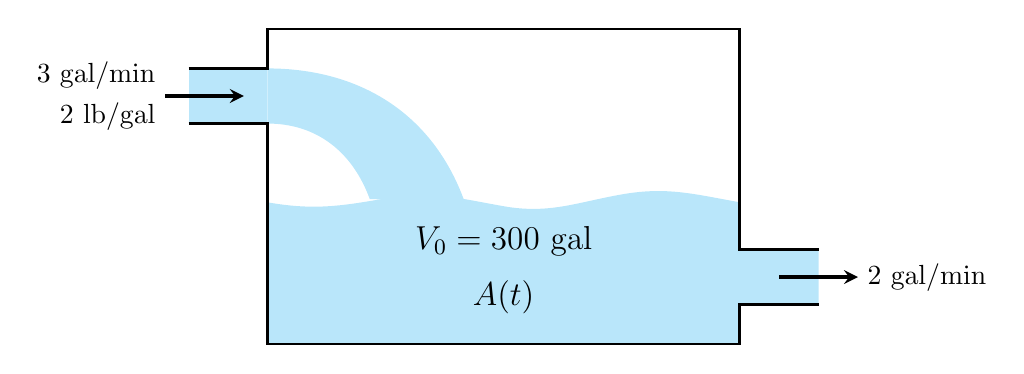
\begin{tikzpicture}

            % Definindo cores
            \definecolor{watercol}{RGB}{185, 230, 250} % Azul claro da água
            \definecolor{textred}{RGB}{220, 0, 0}      % Vermelho para o texto

            % 1. Desenhando a água dentro do tanque (com superfície ondulada)
            \fill[watercol] 
                (0,0) -- (6,0) -- (6,0.5) -- (7,0.5) -- (7,1.2) -- (6,1.2) -- (6,1.8) 
                to[out=170,in=10] (4.5,1.9) 
                to[out=190,in=-10] (3,1.75) 
                to[out=170,in=10] (1.5,1.85) 
                to[out=190,in=-10] (0,1.8) -- cycle;

            % 2. Desenhando a água no cano de entrada e a queda d'água
            \fill[watercol] (-1,2.8) rectangle (0,3.5); % Água no cano
            \fill[watercol] (0,3.5) to[out=0, in=110] (2.5, 1.82) -- (1.3, 1.84) to[out=110, in=0] (0,2.8) -- cycle; % Queda

            % 3. Contorno do tanque (linhas pretas grossas)
            \draw[line width=1] (-1,3.5) -- (0,3.5) -- (0,4) -- (6,4) -- (6,1.2) -- (7,1.2);
            \draw[line width=1] (-1,2.8) -- (0,2.8) -- (0,0) -- (6,0) -- (6,0.5) -- (7,0.5);

            % 4. Textos e Setas - Entrada (Esquerda)
            \node[align=right, anchor=east] at (-1.3, 3.15) {
                $3~\mathrm{gal/min}$ \\[1mm] 
                $2~\mathrm{lb/gal}$
            };
            \draw[->, >=stealth, line width=1.2pt] (-1.3, 3.15) -- (-0.3, 3.15);

            % 5. Textos e Setas - Saída (Direita)
            \draw[->, >=stealth, line width=1.2pt] (6.5, 0.85) -- (7.5, 0.85);
            \node[anchor=west] at (7.5, 0.85) {$2~\mathrm{gal/min}$};

            % 6. Texto central (Quantidade de sal/substância)
            \node at (3, 0.6) {\large $A(t)$};
            \node at (3, 1.3) {\large $V_0=300~\mathrm{gal}$};

            \end{tikzpicture}
            \end{figure}

            \noindent Vamos considerar que a variação da quantidade de sal no tanque seja dada pela diferença entre a taxa de entrada $R_e$ e a taxa de saída $R_s$ do sal. Ou seja, a equação diferencial que descreve o modelo é da forma
            \[\frac{dA}{dt} = R_e - R_s\]
            \noindent A taxa de entrada do sal é dada por
            \[R_e = 3\frac{gal}{min} \times 2\frac{lb}{gal} = 6\frac{lb}{min}\]
            \noindent Já taxa de saída do sal é dada por
            \[R_s = 2\frac{gal}{min} \times C(t)\]
            \noindent Em que $C(t)$ é a concentração da solução dentro do tanque no instante $t$. Podemos descrevê-la tomando a razão entre a quantidade de sal o tanque $A(t)$ e o volume de solução no tanque, da forma $V(t)=V_0+3\dfrac{gal}{min}t-2\dfrac{gal}{min}t=300+t$. Ou seja,
            \[R_s=\frac{2}{300+t}A(t)\]
            \noindent Substituindo na ED, obtemos a expressão de $A(t)$:
            \[\frac{dA}{dt} = 6 - \frac{2}{300+t}A(t)\Rightarrow\boxed{\frac{dA}{dt} + \frac{2}{300+t}A(t) = 6}\]
            
            \noindent\textcolor{blue}{\textbf{Item b)}} Ao modificar a vazão de saída, temos que a taxa de saída do sal passa a ser dada por
            \[R_s = 3.5 \times \frac{A(t)}{300+3t-3.5t}=\frac{7}{600-t}A(t)\]
            \noindent Substituindo na ED, obtemos a expressão de $A(t)$:
            \[\frac{dA}{dt} = 6 - \frac{7}{600-t}A(t)\Rightarrow\boxed{\frac{dA}{dt} + \frac{7}{600-t}A(t) = 6}\]

            \noindent\textcolor{blue}{\textbf{Item c)}} Generalizando o modelo utilizado nos itens anteriores, temos que a taxa de entrada do sal é dada por
            \[R_e = r_e\frac{lb}{gal} \times c_e\frac{gal}{min} = r_ec_e\frac{lb}{min}\]
            \noindent Já a taxa de saída do sal é dada por
            \[R_s = r_s \times \frac{A(t)}{N_0+(r_e-r_s)t}=\frac{r_s}{N_0+(r_e-r_s)t}A(t)\]
            \noindent Dessa forma, substituindo na ED, encontramos
            \[\frac{dA}{dt}=r_ec_e-\frac{r_s}{N_0+(r_e-r_s)t}A(t)\Rightarrow\boxed{\frac{dA}{dt} + \frac{r_s}{N_0+(r_e-r_s)t}A(t) = r_ec_e}\]
        \end{tcolorbox}

        \begin{tcolorbox}[enhanced, breakable, colback=blue!1!white,colframe=blue!75!black,title=\textbf{\hyperlink{quest:ex13}{\hypertarget{resp:ex13}{Exercício 13}}}]
            \noindent\textcolor{blue}{\textbf{Item a)}} A queda de tensão em cada um dos elementos do circuito é
            \[\begin{cases}
                \text{Resistor: } V_R = i(t)R\\
                \text{Indutor: } V_L = L\dfrac{di}{dt}\\
            \end{cases}\]
            \noindent Pela Lei de Kirchoff das Tensões, temos que
            \[\sum V=0\Rightarrow E(t)-V_R-V_L=0\]
            \noindent Substituindo as expressões de $V_R$ e $V_L$, obtemos a equação diferencial que descreve o circuito:
            \[E(t) - i(t)R - L\frac{di}{dt} = 0 \Rightarrow \boxed{L\frac{di}{dt} + Ri(t) = E(t)}\]

            \noindent\textcolor{blue}{\textbf{Item b)}} De modo análogo ao item anterior, podemos escrever as quedas de tensão 
            \[\begin{cases}
                \text{Resistor: } V_R = R\dfrac{dq}{dt}\\
                \text{Capacitor: } V_C = \dfrac{1}{C}q(t)\\
            \end{cases}\]
            \noindent Pela Lei de Kirchoff das Tensões, temos que
            \[\sum V=0\Rightarrow E(t)-V_R-V_C=0\]
            \noindent Substituindo as expressões de $V_R$ e $V_C$, obtemos a equação diferencial que descreve o circuito:
            \[E(t) - R\frac{dq}{dt} - \frac{1}{C}q(t) = 0 \Rightarrow \boxed{R\frac{dq}{dt} + \frac{1}{C}q(t) = E(t)}\]

        \end{tcolorbox}

        \begin{tcolorbox}[enhanced, breakable, colback=blue!1!white,colframe=blue!75!black,title=\textbf{\hyperlink{quest:ex14}{\hypertarget{resp:ex14}{Exercício 14}}}]
            Para auxiliar na resolução do exercício, tomemos como referência o DCL disposto abaixo:
            \begin{figure}[H]
            \centering
            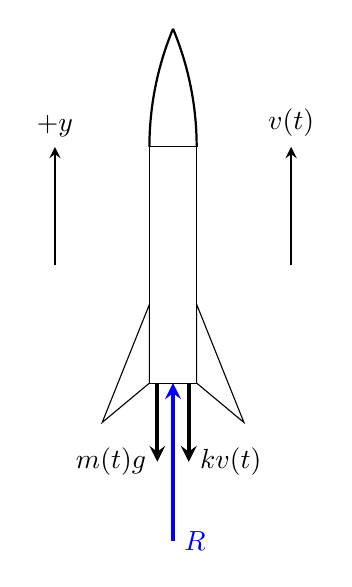
\begin{tikzpicture}[>=stealth]

                \def\Rs{0.3} % Raio da base da ogiva (mesmo do corpo do foguete)
                \def\Lo{1.5} % Comprimento da ogiva
                % Calculando o Raio de Ogiva (Ro)
                \pgfmathsetmacro{\Ro}{(\Lo*\Lo + \Rs*\Rs)/(2*\Rs)}

                % --- Bico Ogival ---
                % Desenha o lado direito da ogiva
                \draw[smooth, variable=\y, domain=1.5:{1.5+\Lo}, thick] 
                    plot ({sqrt(\Ro*\Ro - (\y-1.5)*(\y-1.5)) - (\Ro-\Rs)}, \y);
                % Desenha o lado esquerdo da ogiva
                \draw[smooth, variable=\y, domain=1.5:{1.5+\Lo}, thick] 
                    plot ({-sqrt(\Ro*\Ro - (\y-1.5)*(\y-1.5)) + (\Ro-\Rs)}, \y);

                % 1. Desenhando o foguete (corpo, bico, aletas e chamas)
                %\fill[gray!20] (-0.6, -1.5) rectangle (0.6, 1.5); % Corpo do foguete
                %\fill[gray!50] (-0.6, 1.5) -- (0, 2.5) -- (0.6, 1.5) -- cycle; % Bico
                \draw[smooth] (-0.3, -1.5) -- (-0.9, -2) -- (-0.3, -0.5) -- cycle; % Aleta esquerda
                \draw[smooth] (0.3, -1.5) -- (0.9, -2) -- (0.3, -0.5) -- cycle; % Aleta direita
                %\fill[orange!80!red] (-0.4, -1.5) -- (0, -2.5) -- (0.4, -1.5) -- cycle; % Fogo/Exaustão
                \draw[smooth] (-0.3, -1.5) rectangle (0.3, 1.5); % Contorno do corpo
                %\draw[thick] (-0.6, 1.5) -- (0, 2.5) -- (0.6, 1.5); % Contorno do bico

                % 2. Eixo de Referência (Direção Positiva)
                \draw[->, thick] (-1.5, 0) -- (-1.5, 1.5) node[above] {$+y$};

                % 3. Vetores de Força (saindo do CM)
                
                % Força de Propulsão (R) - Para cima
                \draw[->, line width=1.5pt, blue] (0, -3.5) node[right] {$R$} -- (0, -1.5) ;

                % Força Peso (m(t)g) - Para baixo (deslocado ligeiramente para a esquerda para não sobrepor)
                \draw[->, line width=1.5pt] (-0.2, -1.5) -- (-0.2, -2.5) node[left] {$m(t)g$};

                % Força de Resistência do ar (kv) - Para baixo (deslocado ligeiramente para a direita)
                \draw[->, line width=1.5pt] (0.2, -1.5) -- (0.2, -2.5) node[right] {$kv(t)$};

                % 4. Vetor Velocidade (ao lado, para indicar o movimento)
                \draw[->, thick] (1.5, 0) -- (1.5, 1.5) node[above] {$v(t)$};

            \end{tikzpicture}
            \end{figure}

            \noindent A força resultante que atua sobre o foguete é tal que 
            \[F=R-m(t)g-kv(t)\]
            \noindent Desenvolvendo a Segunda Lei de Newton, temos que
            \[F=\frac{d}{dt}(mv)=\frac{dm}{dt}v(t)+m\frac{dv}{dt}\]
            \noindent Assim, substituindo a primeira expressão na segunda, encontramos que
            \[R-m(t)g-kv(t) = \frac{dm}{dt}v(t)+m\frac{dv}{dt}\Rightarrow\boxed{m\frac{dv}{dt} + \left(k+\frac{dm}{dt}\right)v(t) = R - m(t)g}\]

            Sendo esse o modelo matemático que descreve $v(t)$.

        \end{tcolorbox}

        \begin{tcolorbox}[enhanced, breakable, colback=blue!1!white,colframe=blue!75!black,title=\textbf{\hyperlink{quest:ex15}{\hypertarget{resp:ex15}{Exercício 15}}}]
            \noindent\textcolor{blue}{\textbf{Item a)}} Vamos tomar a primeira derivada da expressão de $m(t)$:
            \[\frac{dm}{dt}=\frac{dm_p}{dt}+\frac{dm_v}{dt}+\frac{dm_f}{dt}\]
            \noindent Se $m_p$ e $m_f$ são constantes, então
            \[\frac{dm}{dt}=0+0+\frac{dm_f}{dt}\Rightarrow\boxed{\frac{dm}{dt}=\frac{dm_f}{dt}}\]
            \noindent o que prova que a taxa de variação da massa total é igual à taxa de variação da massa de combustível.

            \noindent\textcolor{blue}{\textbf{Item b)}} Se o foguete consome combustível a uma taxa constante $\lambda$, então a massa de combustível pode ser descrita pela relação linear
            \[m_f(t)=m_f(0)-\lambda t\]
            Utilizando essa relação na expressão de $m(t)$, temos que
            \[m(t)=m_p+m_v+m_f(0)-\lambda t\]
            Sabendo que $m_p+m_v+m_f(0)=m(0)=m_0$, obtemos a relação
            \[m(t)=m_0-\lambda t\]
            Usando essa relação na expressão do \hyperlink{resp:ex14}{Exercício 14}, temos
            \[\boxed{(m_0-\lambda t)\frac{dv}{dt}+(k-\lambda)v(t)=R-(m_0-\lambda t)g}\]

            \noindent\textcolor{blue}{\textbf{Item c)}} Queremos achar o instante em que a função $m_f(t)$ definida no item b) atinge $0$. Nesse sentido, temos
            \[m_f(t_b)=0=m_f(0)-\lambda t_b\Rightarrow\boxed{t_b=\frac{m_f(0)}{\lambda}}\]
            \noindent igual à expressão apresentada no enunciado.
        \end{tcolorbox}


\end{document}